\section{Methodology}
\label{sec:methodology}
In this section, the methodology proposed in this study is presented. Firstly, approach overview is described from a high-level perspective. Then, each stage in the methodology is presented together with their importance in the study, mathematical representations and definitions; and black-box diagrams. In the last section of this chapter, implementation details of this methodology in ProM framework is explained in detail with a software architecture overview.

\subsection{Approach Overview}
\label{subsec:approach-overview}
The approach proposed in this study consists of four main stages visualized in Figure~\ref{fig:approach-overview}. Firstly, in \textit{Process Model Mining}, process models are extracted from event logs for each organization with a user specified noise threshold. Secondly, in \textit{Performance Indicator Analysis}, event logs are replayed on process models and performance indicators are calculated for each organization then using these indicators, organizations are clustered based on how well they are operating. Thirdly, in \textit{Mismatch Pattern Analysis}, differences between process models of organizations are extracted with well-established mismatch patterns. Finally, in \textit{Recommendation Generation}, using the performance indicator clusterings and differences between process models, a set of recommendations for each organization is generated. In the following sections, each stage will be explained in detail with their mathematical backgrounds.

\begin{figure}
  \centering
  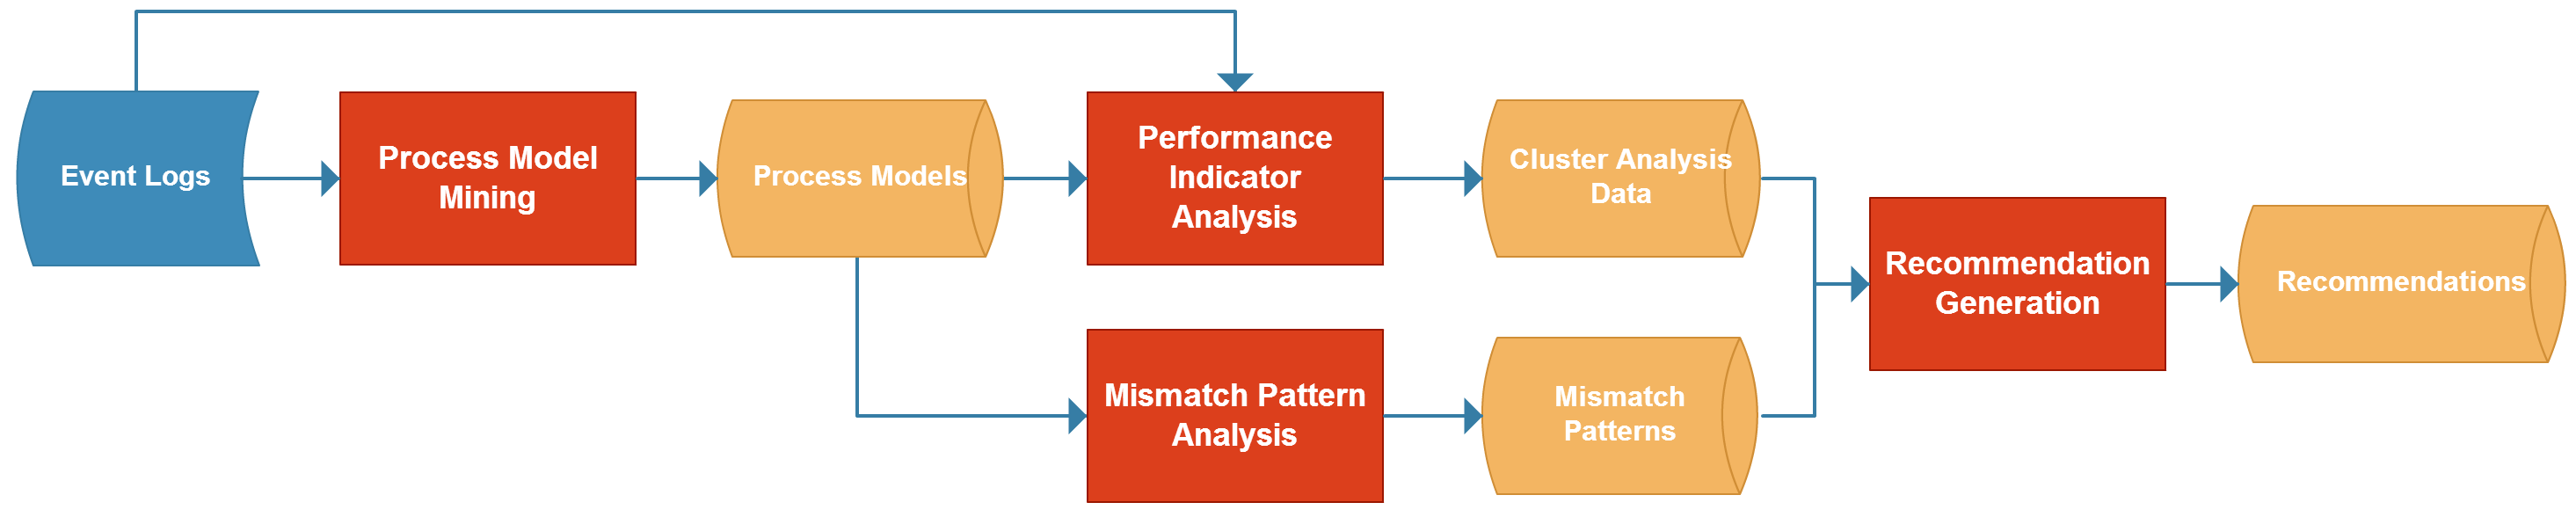
\includegraphics[width=\textwidth]{4_methodology/approach-overview}
  \caption{Overview of Methodology}
  \label{fig:approach-overview}
\end{figure}